\section{Brugervejledning}

Når du åbner appen vil du blive mødt med forsiden for den nuværende sæson. Her har du mulighed for at designe og planlægge din have. Som udgangspunkt, er haven delt op i to: udendørs køkkenhave og drivhus. Trykker du på en af kategorierne, vil som førstegangsbruger blive mødt med en tom have.

\subsection{Design din have}

\begin{minipage}{0.4\textwidth}
\begin{figure}[H]
    \centering
    \frame{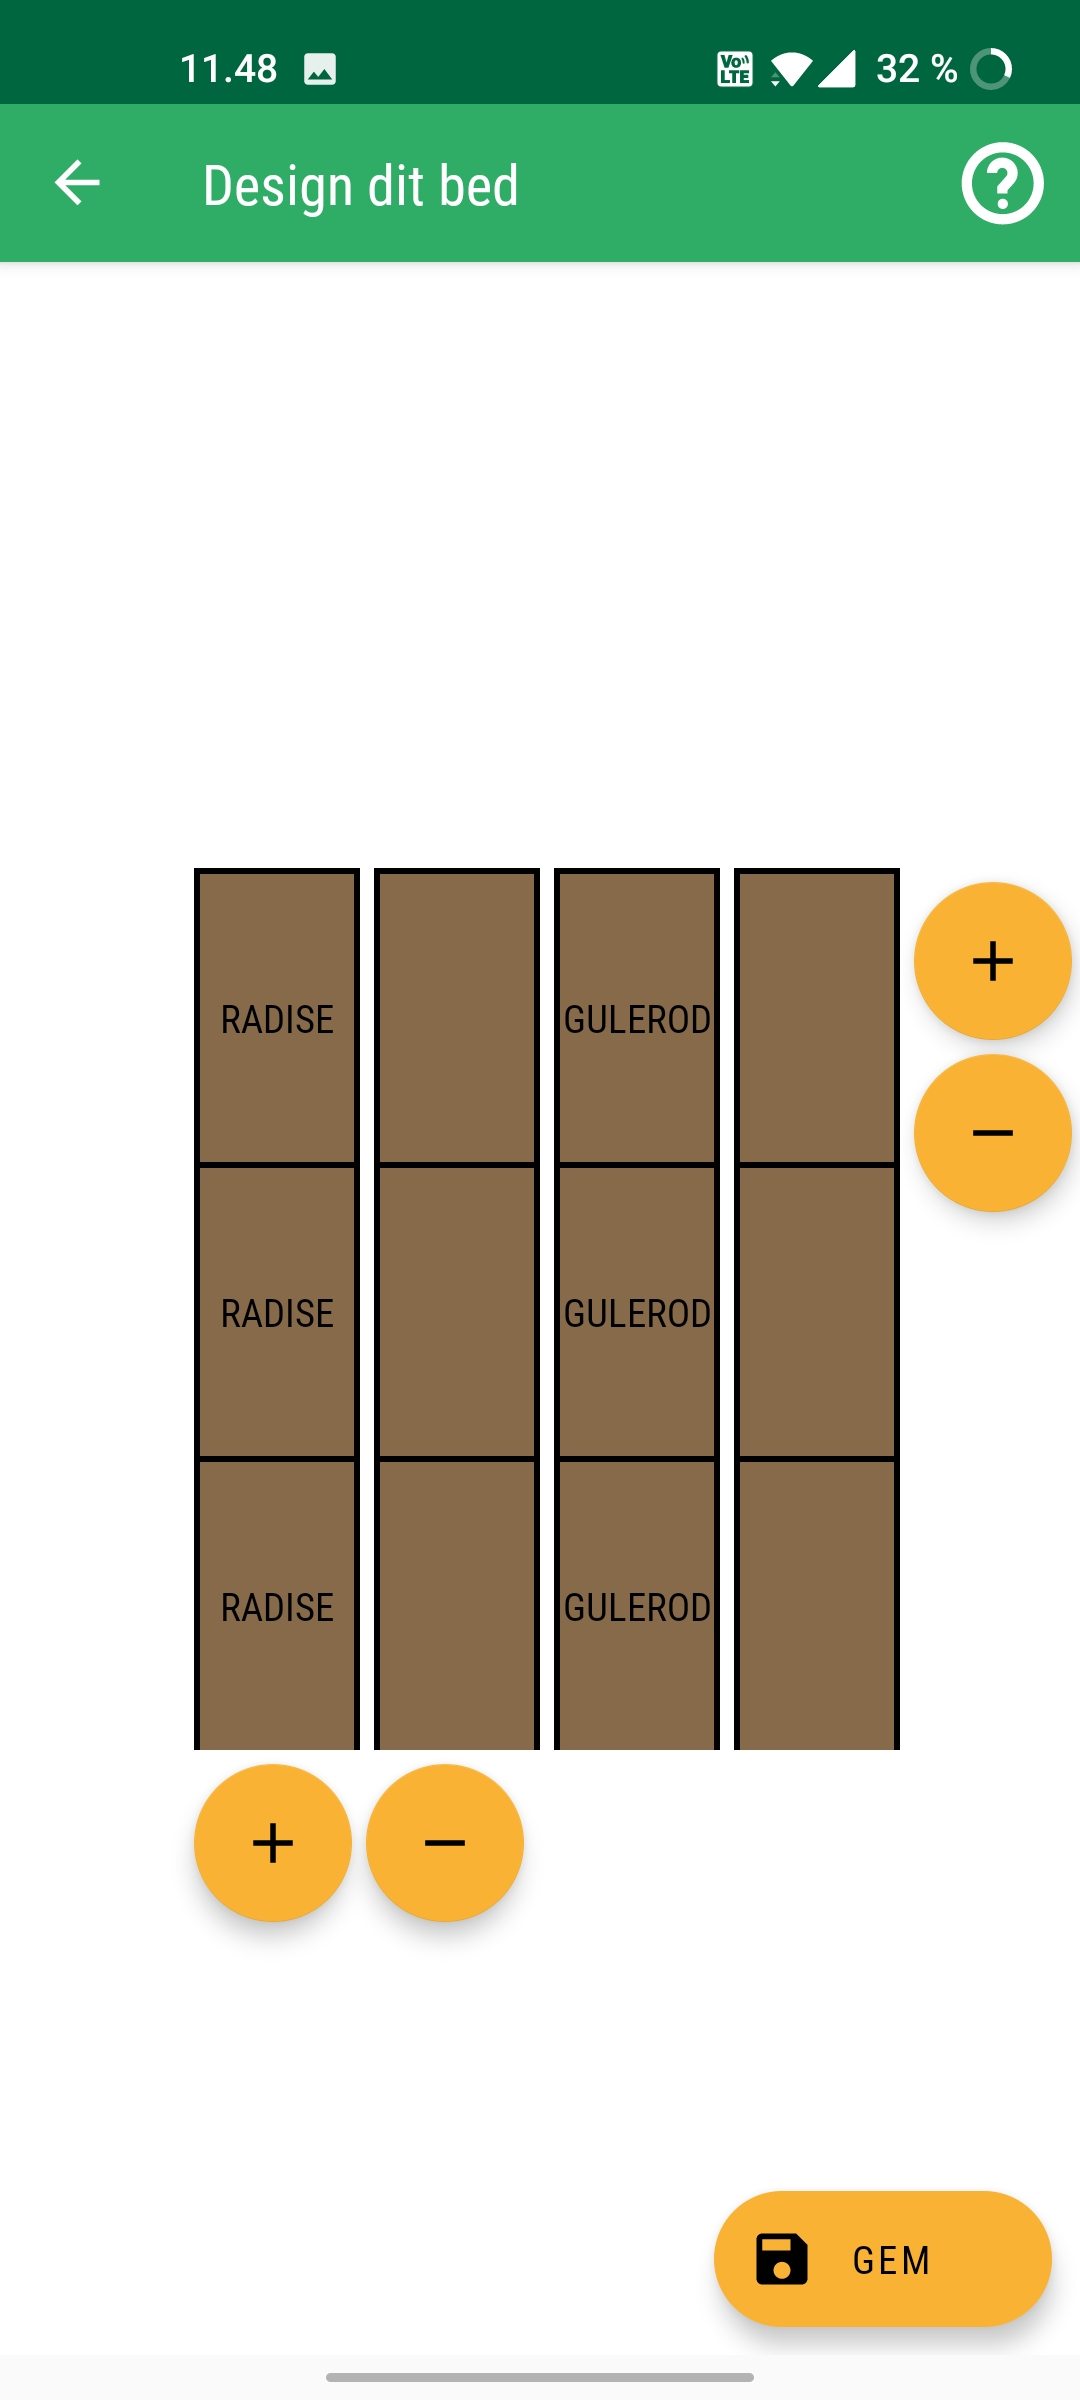
\includegraphics[width=\textwidth]{img/screenshot-nyt-bed.jpg}}
    \caption{Opret et nyt bed eller område}
\end{figure}
\end{minipage} \hfill
\begin{minipage}{0.55\textwidth}    
Når du har valgt 'Udendørs' eller 'Drivhus' kan du se og oprette bede, eller andre forskellige områder du ønsker at repræsentere i appen. Tryk på plus-knappen nede i hjørnet for at komme i gang.
Hvert felt i bedet kan indeholde en plante. Tryk på feltet for at få en liste over planter og vælg, hvilken du ønsker at placere. Du kan ændre bedets størrelse på plus- og minus-knapperne til højre og for neden. Hvis dit bed ikke er firkantet, anbefaler vi, at du laver bedet større end dit fysiske bed og blot udfylder de felter, der bedst repræsenterer en anden facon. Når du er færdig kan du klikke på gem og navngive dit bed. En måde, at navngive bede på, kan være at bruge typen af planter i bedet.
\end{minipage} 

\begin{minipage}{0.4\textwidth}
\begin{figure}[H]
    \centering
    \frame{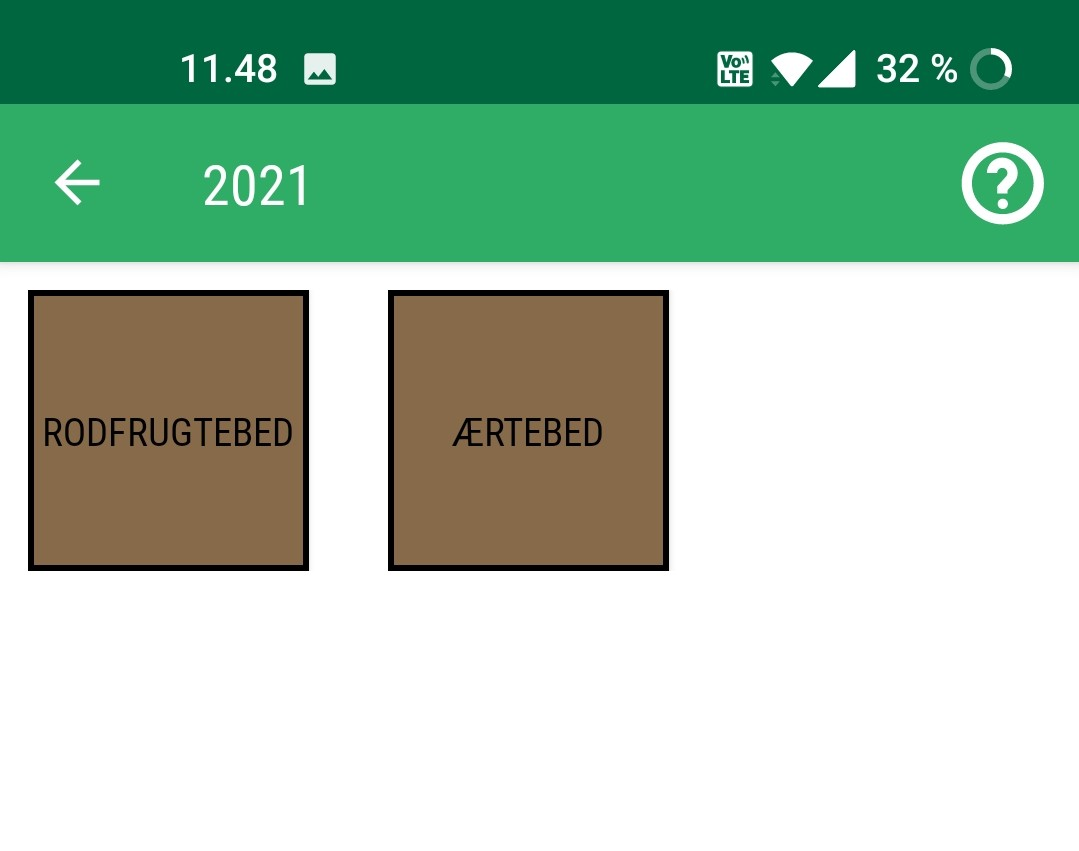
\includegraphics[width=\textwidth]{img/screenshot-oversigt-bede.jpg}}
    \caption{Oversigt over bede}
\end{figure}
\end{minipage} \hfill
\begin{minipage}{0.5\textwidth}
Når du har oprettet din have kan du se dem i den oversigt, der før var tom.
For at få det til at ligne din egen have mest muligt, kan du holde inde på et bed og trække i det for at skifte bedenes rækkefølge. Dette kan også hjælpe appen til at holde styr på sædskifte. Læs mere om dette under sædskifte.
\end{minipage}

\subsection{Planlæg kommende sæsoner og se historik}
\begin{minipage}{0.4\textwidth}
\begin{figure}[H]
    \centering
    \frame{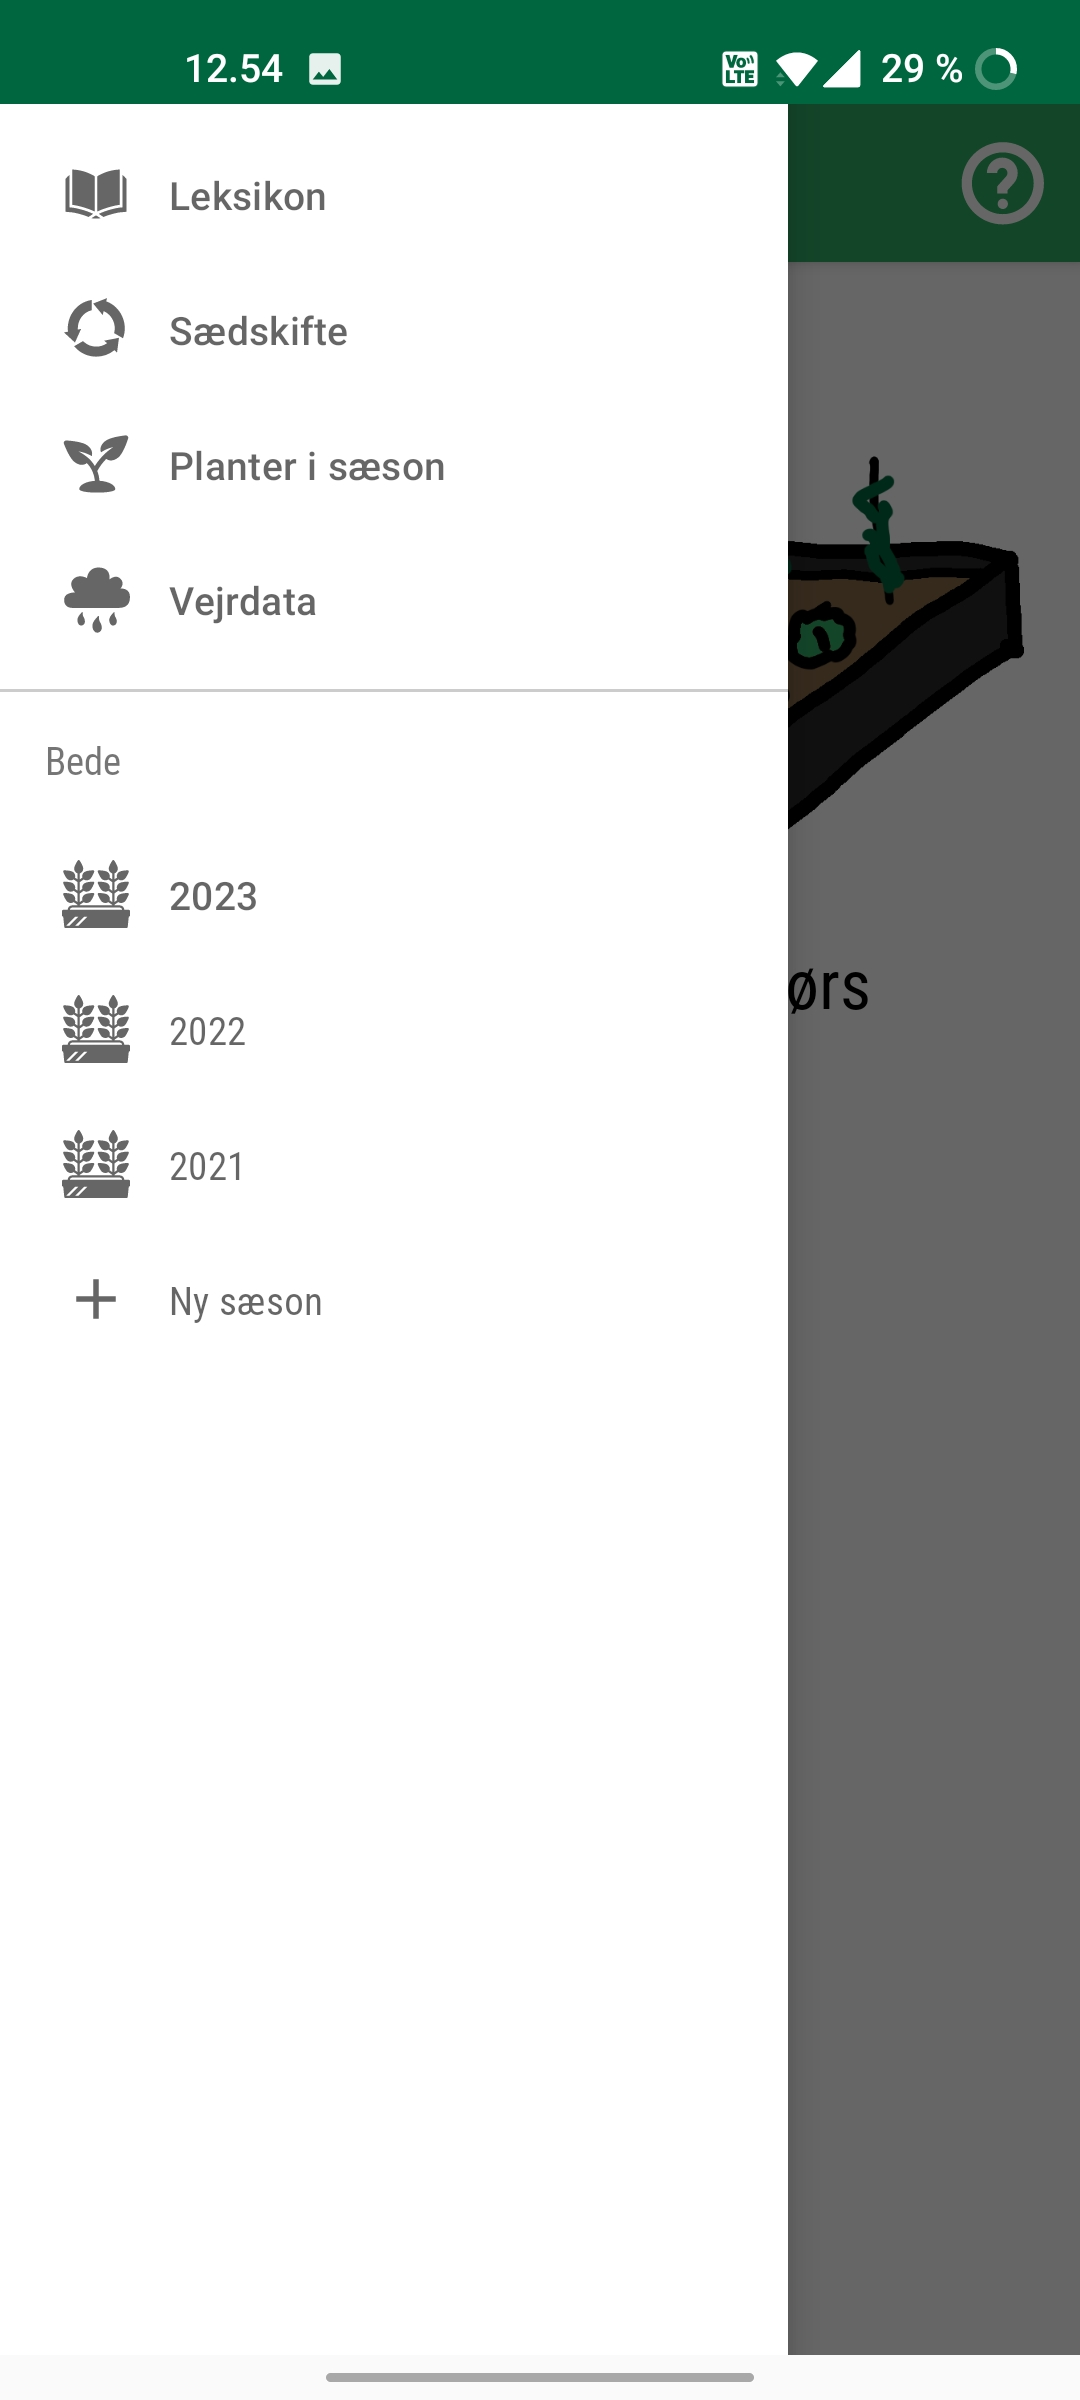
\includegraphics[width=\textwidth]{img/screenshot-sidemenu.jpg}}
    \caption{Opret et nyt bed eller område}
\end{figure}
\end{minipage} \hfill
\begin{minipage}{0.55\textwidth}
I side-menuen, som kan åbnes øverst til venstre, kan du se en oversigt over alle de oprettede sæsoner. Når du åbner appen første gang, vil der automatisk være oprettet en sæson for det nuværende årstal. Du kan oprette en ny sæson ved at trykke på "Ny sæson", og indtaste hvilket årstal, sæsonen skal repræsentere. Du kan bruge denne funktion til at planlægge i forvejen, og dermed f.eks. oprette næste sæson i god tid. Du kan også vælge at oprette de nye sæsoner efterhånden som du når dertil. De gamle sæsoner vil altid være gemt, og det vil derfor være nemt at trykke tilbage og se, hvordan din have så ud tidligere.
\end{minipage} 

\subsection{Se og opret planter}

\subsection{Få styr på sædskifte}

\subsection{Hvilke planter er i sæson?}

\subsection{Vurder vanding i forhold til lokalvejret}
